\section{Sliding window protocol}
In \autoref{subsec:data-format} it was decided that the format of timestamps would be an integer from 0-255, where 0 to 20 would be considered as newer timestamps than 235 to 255.
However, if all the timestamps between 0 to 20, there would not be any updates until it has looped to a number between 0 and 20 and sent new updates.
To find a better solution to sliding window protocol was researched.
\\\\
Sliding window protocols are often used where reliable data is required.
Whenever the senders has sent the window sized packets, it waits for acknowledgement from the receiver before it sends new packets.
Each packet gets a sequence number and the acknowledgement sends back this number.
By doing this the receiver can keep track of the packets, remove duplicates, identify missing packets and know which order is the correct one.
\\\\
On \autoref{fig:sliding-window} there is an illustration of an ideal sliding window, where W is the window size, and n is the number of packets that has not been acknowledged.
The sender will send the packets until the window is full and then wait for an acknowledgement from the sent packets.
\begin{figure}[H]
    \centering
    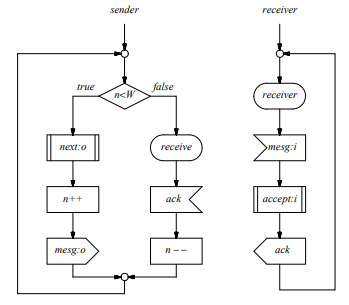
\includegraphics[width=0.6\linewidth]{window-protocol-illustration.PNG}
    \caption{Sliding window protocol without timeouts or message loss \cite{design-and-validation-of-computer-protocols}.}
    \label{fig:sliding-window}
\end{figure}
\noindent
For our project reliable data in the format of goal zones and goal score is important, however the player position is not important that it is reliable.
This is due to our prioritization that the update rate is higher and hereby we previously choose to use UDP in \autoref{subsubsec:choosing-between-udp-or-tcp}.
With Sliding Window protocol a player position would be retransmitted if it previously failed, and these positions quickly become outdated.
TCP also already uses sliding window for flow control so for goal zones and goal score it is not necessary to implement, as these use TCP \cite{ibm:sliding-window}.
